\section{Cálculo de Correas}

Diseñar las correas de cubierta y laterales de chapa doblada F-24, no se utilizarán tillas para el cálculo de las mismas, la estructura posee las siguientes características.

\begin{itemize}
\item Las acciones y dimensiones para correas de techo son.
\begin{align*}
& \text{Chapa} \rightarrow 7 \frac{Kg}{m^2}\\
& \text{Aislación} \rightarrow 1.5 \frac{Kg}{m^2}\\
& \text{Sujeción} \rightarrow 1.5 \frac{Kg}{m^2}\\
& \text{Correas} \rightarrow  4 \frac{Kg}{m^2}\\
& \text{Peso propio} \rightarrow  g = 7 \frac{Kg}{m^2}+1.5 \frac{Kg}{m^2}+1.5 \frac{Kg}{m^2}+4 \frac{Kg}{m^2} = 14 \frac{Kg}{m^2}
\end{align*}
\begin{align*}
& g=14 \frac{Kg}{m^2} \quad \text{Peso propio}\\
& p=96 \frac{Kg}{m^2} \quad \text{Sobrecarga}\\
& q_w=144 \frac{Kg}{m^2} \quad \text{Viento}\\
& s= 1m \quad \text{Separación entre correas} \\
& l= 5m \quad \text{Separación entre pórticos} \\
& \alpha = 14.35\textsuperscript{o} \quad \text{Inclinación de la cubierta}
\end{align*}

\item Las acciones y dimensiones para correas laterales son.
\begin{align*}
& g=14 \frac{Kg}{m^2} \quad \text{Peso propio}\\
& q_w=214 \frac{Kg}{m^2} \quad \text{Viento}\\
& s= 1.20m \quad \text{Separación entre correas} \\
& l= 5m \quad \text{Separación entre pórticos}
\end{align*}
\end{itemize}

\newpage
\begin{enumerate}
\item \underline{Correas de Techo. Caso Sin Tillas}\\
\begin{itemize}
\item El primer estado de carga corresponde a peso propio + sobrecarga.

\begin{figure}[H]
\begin{center}
     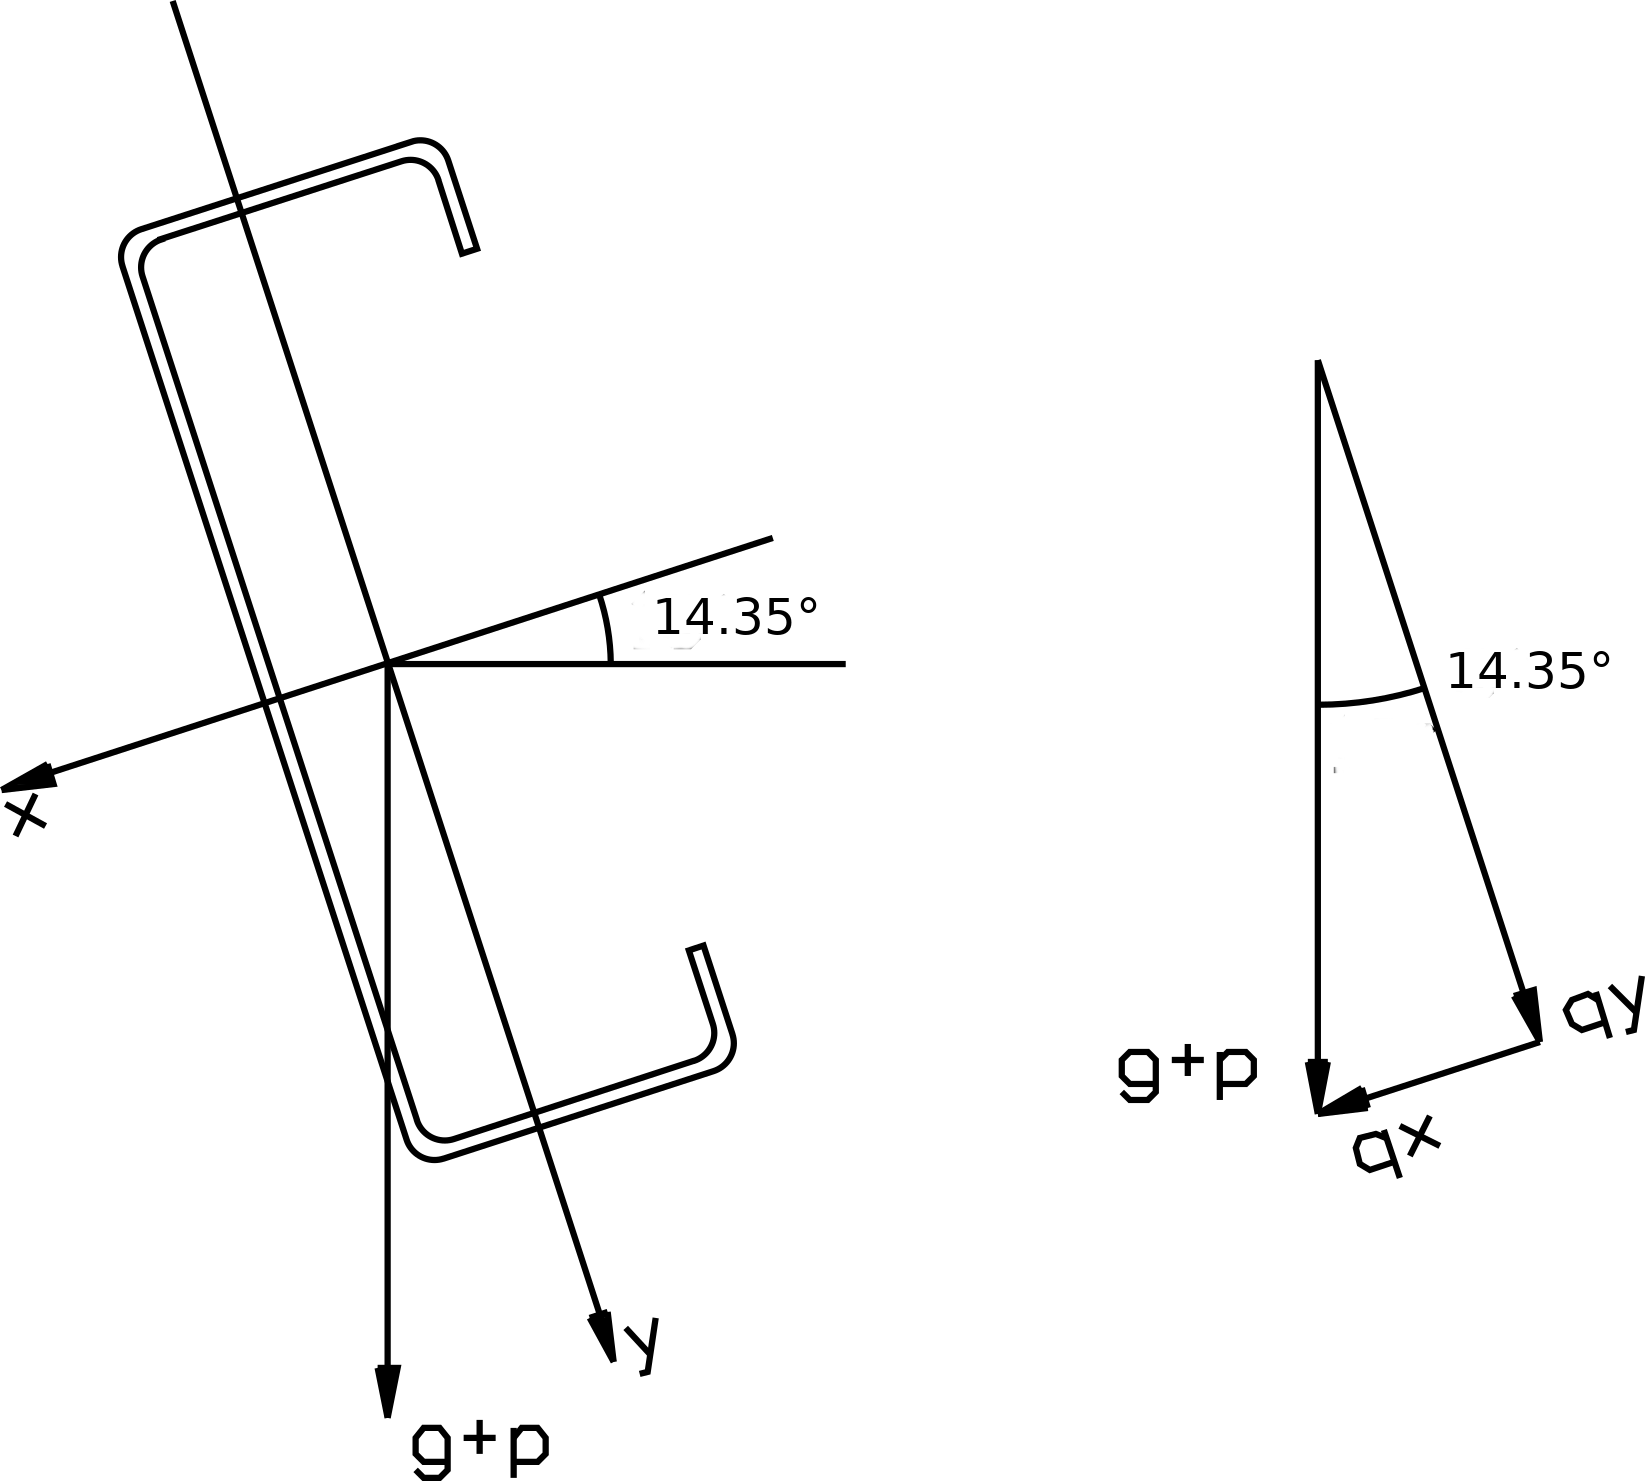
\includegraphics[scale = 1]{chapters/chapter_3/images/figura1.png}
\caption{Correa de techo sin tillas - Estado: peso propio + sobrecarga}
\end{center}
\end{figure}

$$q= (g+p)\cdot s = (14 \frac{Kg}{m^2}+96 \frac{Kg}{m^2}) \cdot 1m = \framebox{$110 \frac{Kg}{m}$}$$
Descomponiendo la resultante en las direcciones $x$ e $y$ tenemos:
\begin{align*}
& q_x=q \cdot Sen \alpha= 110 \frac{Kg}{m} \cdot Sen(14.35\textsuperscript{o})= \framebox{$27.26 \frac{Kg}{m}$}\\
& q_y=q \cdot Cos \alpha= 110 \frac{Kg}{m} \cdot Cos(14.35\textsuperscript{o})= \framebox{$106.56 \frac{Kg}{m}$}
\end{align*}

Procedemos a calcular los momentos en el centro de la luz, producidos por cada una de estas cargas lineales, suponemos que las correas se encuentran simplemente apoyadas.
\begin{align*}
& M_x= \frac{q_y \cdot l^2}{8} = \frac{106.56 \frac{Kg}{m} \cdot (5m)^2}{8} = \framebox{$333.02 Kg.m$} \\
& M_y= \frac{q_x \cdot l^2}{8} = \frac{27.26 \frac{Kg}{m} \cdot (5m)^2}{8} = \framebox{$85.19 Kg.m$}
\end{align*}

\newpage
\item El segundo estado de carga corresponde a peso propio + viento.

\begin{figure}[H]
\begin{center}
     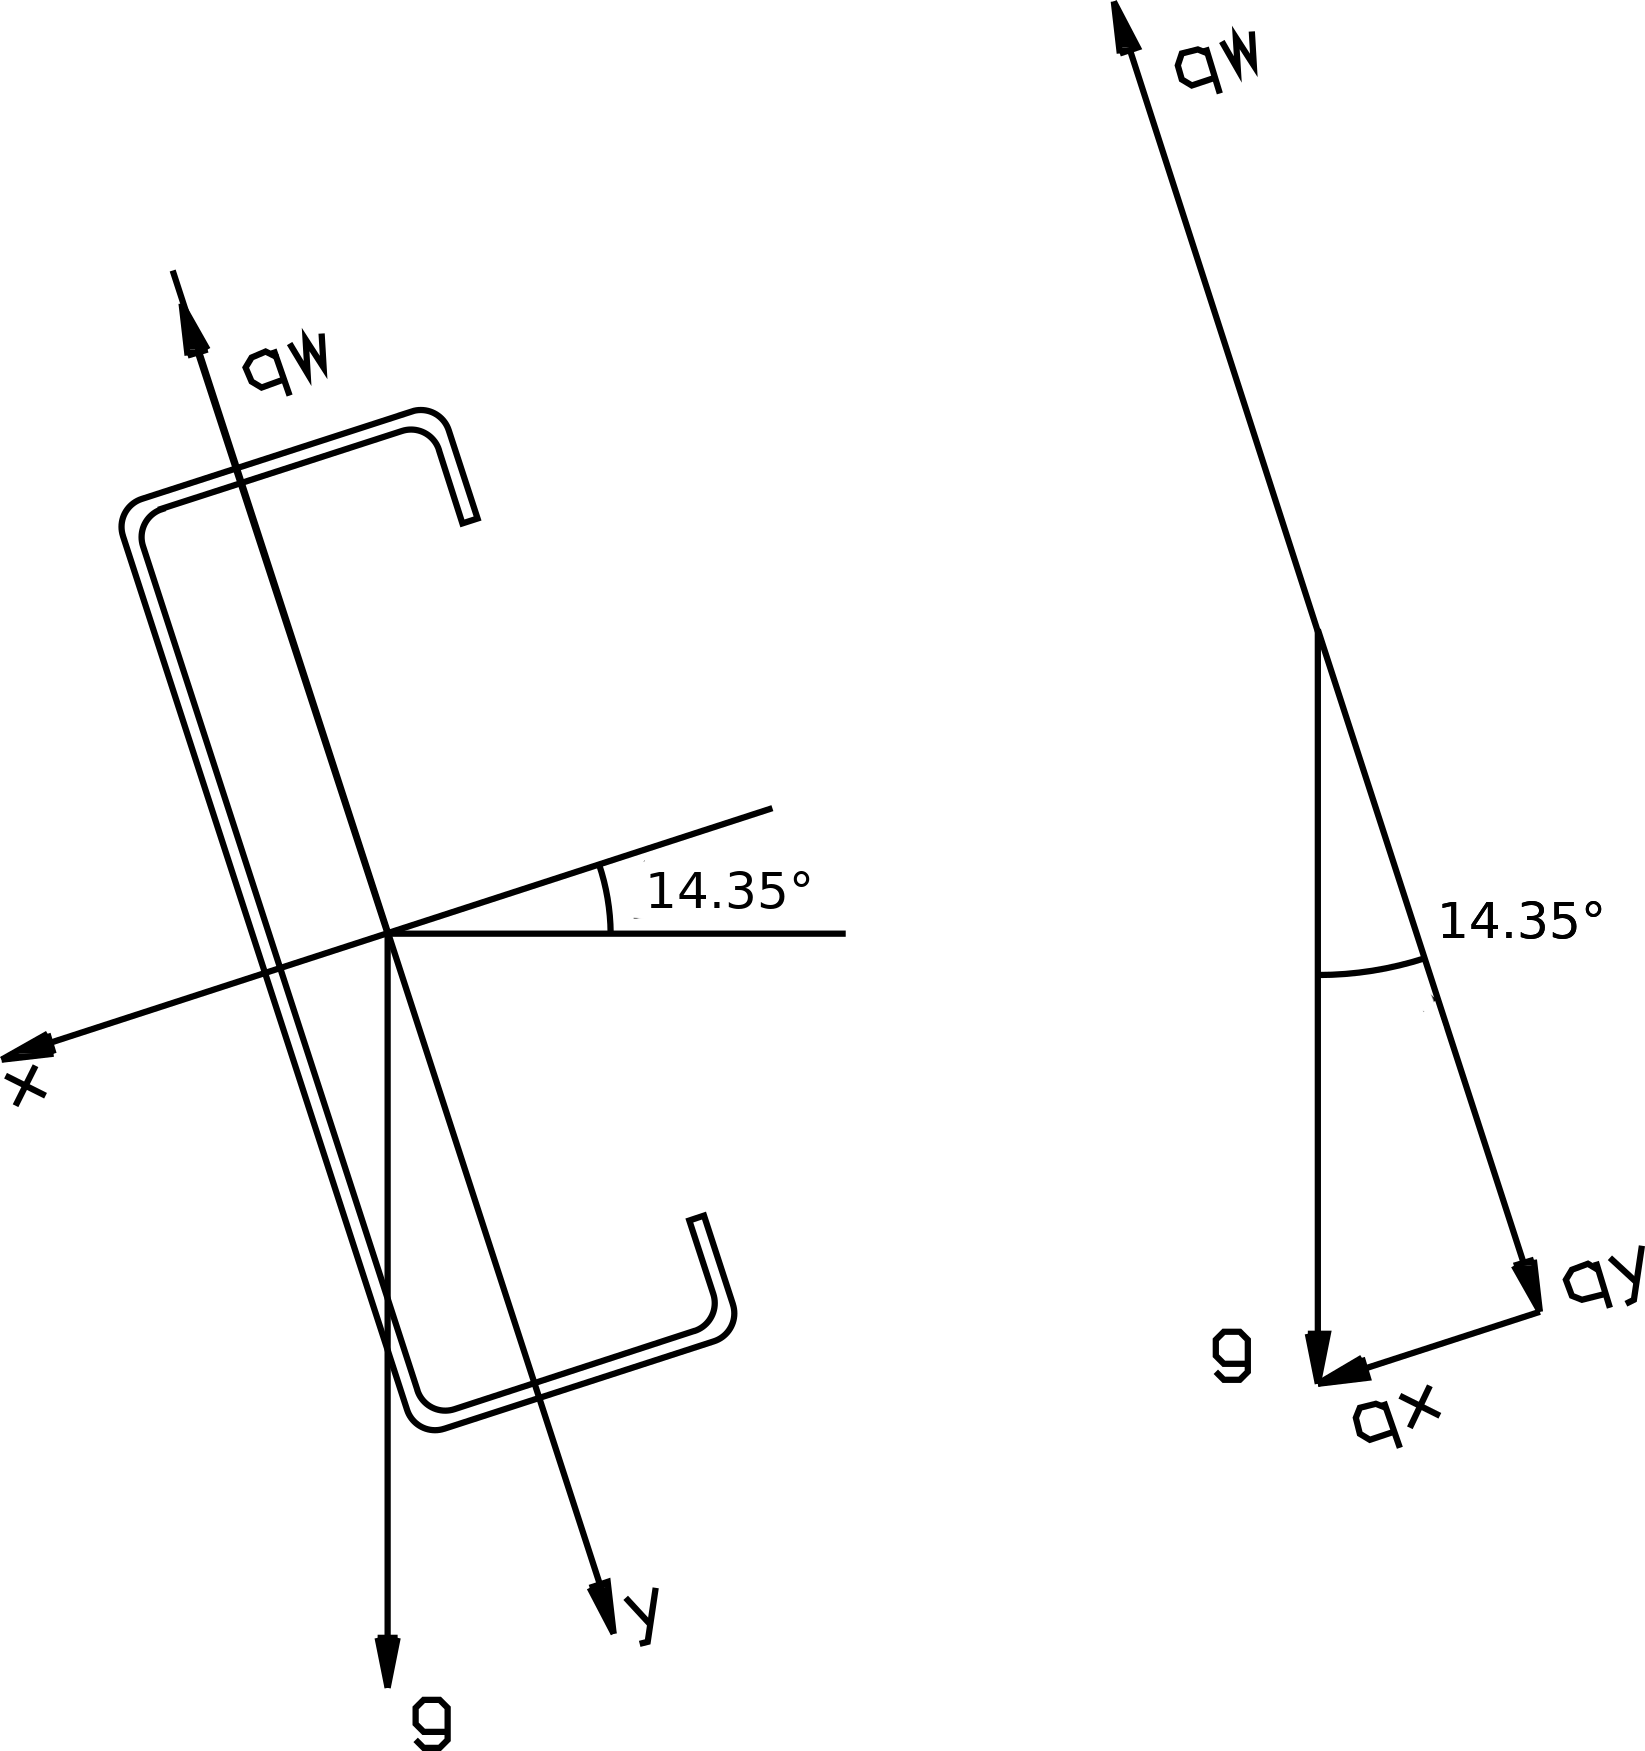
\includegraphics[scale = 1]{chapters/chapter_3/images/figura2.png}
\caption{Correa de techo sin tillas - Estado: peso propio + viento}
\end{center}
\end{figure}

Descomponiendo la resultante en las direcciones $x$ e $y$ tenemos:
\begin{align*}
& q_x=g \cdot Sen \alpha \cdot s = 14 \frac{Kg}{m^2} \cdot Sen(14.35\textsuperscript{o}) \cdot 1m= \framebox{$3.46 \frac{Kg}{m}$}\\
& q_y=(q_w - g \cdot Cos \alpha) \cdot s = (144 \frac{Kg}{m^2} - 14 \frac{Kg}{m^2} \cdot Cos(14.35\textsuperscript{o}) \cdot 1m= \framebox{$130.43 \frac{Kg}{m}$}
\end{align*}

Procedemos a calcular los momentos en el centro de la luz, producidos por cada una de estas cargas lineales, suponemos que las correas se encuentran simplemente apoyadas.

\begin{align*}
& M_x= \frac{q_y \cdot l^2}{8} = \frac{130.43 \frac{Kg}{m} \cdot (5m)^2}{8} = \framebox{$407.59 Kg.m$} \\
& M_y= \frac{q_x \cdot l^2}{8} = \frac{3.46 \frac{Kg}{m} \cdot (5m)^2}{8} = \framebox{$10.81 Kg.m$}
\end{align*}

\item Tension admisible.\\
Dado que se utiliza acero F-24, tenemos según el reglamento CIRSOC 301 una tensión de fluencia $\sigma_{fl}=2400 \frac{Kg}{cm^2}$ y tomando un coeficiente de seguridad $\gamma = 1.6$ , se obtiene una tensión admisible de:
$$\sigma_{adm}= \frac{\sigma_{fl}}{\gamma} = \frac{2400 \frac{Kg}{cm^2}}{1.6} = \framebox{$1500 \frac{Kg}{cm^2}$}$$

\newpage
\item Selección de la correa.\\
Adoptamos un perfil \framebox{C 180-70-25-3.2} de chapa doblada, con las siguientes características:
\begin{align*}
& W_x= 61.027 cm^3 \\
& W_y= 15.882 cm^3 \\
& J_x= 549.239 cm^4 \\
& J_y= 75.347 cm^4
\end{align*}

\item Verificamos las tensiones para ambos estados de carga.\\
\underline{Estado de carga 1: peso propio + sobrecarga}
\begin{align*}
& \sigma_x=\frac{M_x}{W_x} = \frac{33302 Kg.cm}{61.027 cm^3} = 545.69 \frac{Kg}{cm^2}\\
& \sigma_y=\frac{M_y}{W_y} = \frac{8519 Kg.cm}{15.882 cm^3} = 536.39 \frac{Kg}{cm^2}\\
& \sigma_t= \sigma_x + \sigma_y = 545.69 \frac{Kg}{cm^2} + 536.39 \frac{Kg}{cm^2} = \framebox{$1082.08 \frac{Kg}{cm^2}$}\\
& \sigma_t < \sigma_{adm}\\
& 1082.08 \frac{Kg}{cm^2} < 1500 \frac{Kg}{cm^2} \Rightarrow \text{Verifica} \quad \surd
\end{align*}

\underline{Estado de carga 2: peso propio + viento}
\begin{align*}
& \sigma_x=\frac{M_x}{W_x} = \frac{40759 Kg.cm}{61.027 cm^3} = 667.88 \frac{Kg}{cm^2}\\
& \sigma_y=\frac{M_y}{W_y} = \frac{1081 Kg.cm}{15.882 cm^3} = 68.06 \frac{Kg}{cm^2}\\
& \sigma_t= \sigma_x + \sigma_y = 667.88 \frac{Kg}{cm^2} + 68.06 \frac{Kg}{cm^2} = \framebox{$735.94 \frac{Kg}{cm^2}$}\\
& \sigma_t < \sigma_{adm}\\
& 735.94 \frac{Kg}{cm^2} < 1500 \frac{Kg}{cm^2} \Rightarrow \text{Verifica} \quad \surd
\end{align*}

\item Verificamos las deformaciones para ambos estados de carga.\\
La flecha admisible de cumplir $f < \frac{l}{300} \Rightarrow f < \frac{5m}{300} \Rightarrow f < 1.66cm$\\
Para el cálculo de la flecha utilizaremos la expresión $f= \frac{5}{384} \cdot \frac{q \cdot l^4}{E \cdot J}$\\

\underline{Estado de carga 1: peso propio + sobrecarga}
\begin{align*}
& f_x=\frac{5}{384} \cdot \frac{q_x \cdot l^4}{E \cdot J_y}\\
& f_x=\frac{5}{384} \cdot \frac{0.2726 \frac{Kg}{cm} \cdot (500cm)^4}{2100000 \frac{Kg}{cm^2} \cdot 75.347 cm^4} = 1.40cm\\
& f_y=\frac{5}{384} \cdot \frac{q_y \cdot l^4}{E \cdot J_x}\\
& f_y=\frac{5}{384} \cdot \frac{1.0656 \frac{Kg}{cm} \cdot (500cm)^4}{2100000 \frac{Kg}{cm^2} \cdot 549.239 cm^4} = 0.75cm\\
& f = \sqrt{f_x^2+f_y^2} = \sqrt{(1.40cm)^2+(0.75cm)^2} = \framebox{$1.59cm$}\\
& f < f_{adm}\\
& 1.59cm < 1.66cm \Rightarrow \text{Verifica} \quad \surd
\end{align*}

\underline{Estado de carga 2: peso propio + viento}
\begin{align*}
& f_x=\frac{5}{384} \cdot \frac{q_x \cdot l^4}{E \cdot J_y}\\
& f_x=\frac{5}{384} \cdot \frac{0.0346 \frac{Kg}{cm} \cdot (500cm)^4}{2100000 \frac{Kg}{cm^2} \cdot 75.347 cm^4} = 0.18cm\\
& f_y=\frac{5}{384} \cdot \frac{q_y \cdot l^4}{E \cdot J_x}\\
& f_y=\frac{5}{384} \cdot \frac{1.3043 \frac{Kg}{cm} \cdot (500cm)^4}{2100000 \frac{Kg}{cm^2} \cdot 549.239 cm^4} = 0.92cm\\
& f = \sqrt{f_x^2+f_y^2} = \sqrt{(0.18cm)^2+(0.92cm)^2} = \framebox{$0.94cm$}\\
& f < f_{adm}\\
& 0.94cm < 1.66cm \Rightarrow \text{Verifica} \quad \surd
\end{align*}
Por lo tanto verifica el requerimiento de deformación especificado en el reglamento.\\
\end{itemize}

\newpage
\item \underline{Correas Laterales.}\\
\begin{itemize}

\item El estado de carga corresponde a peso propio + viento.

\begin{figure}[H]
\begin{center}
     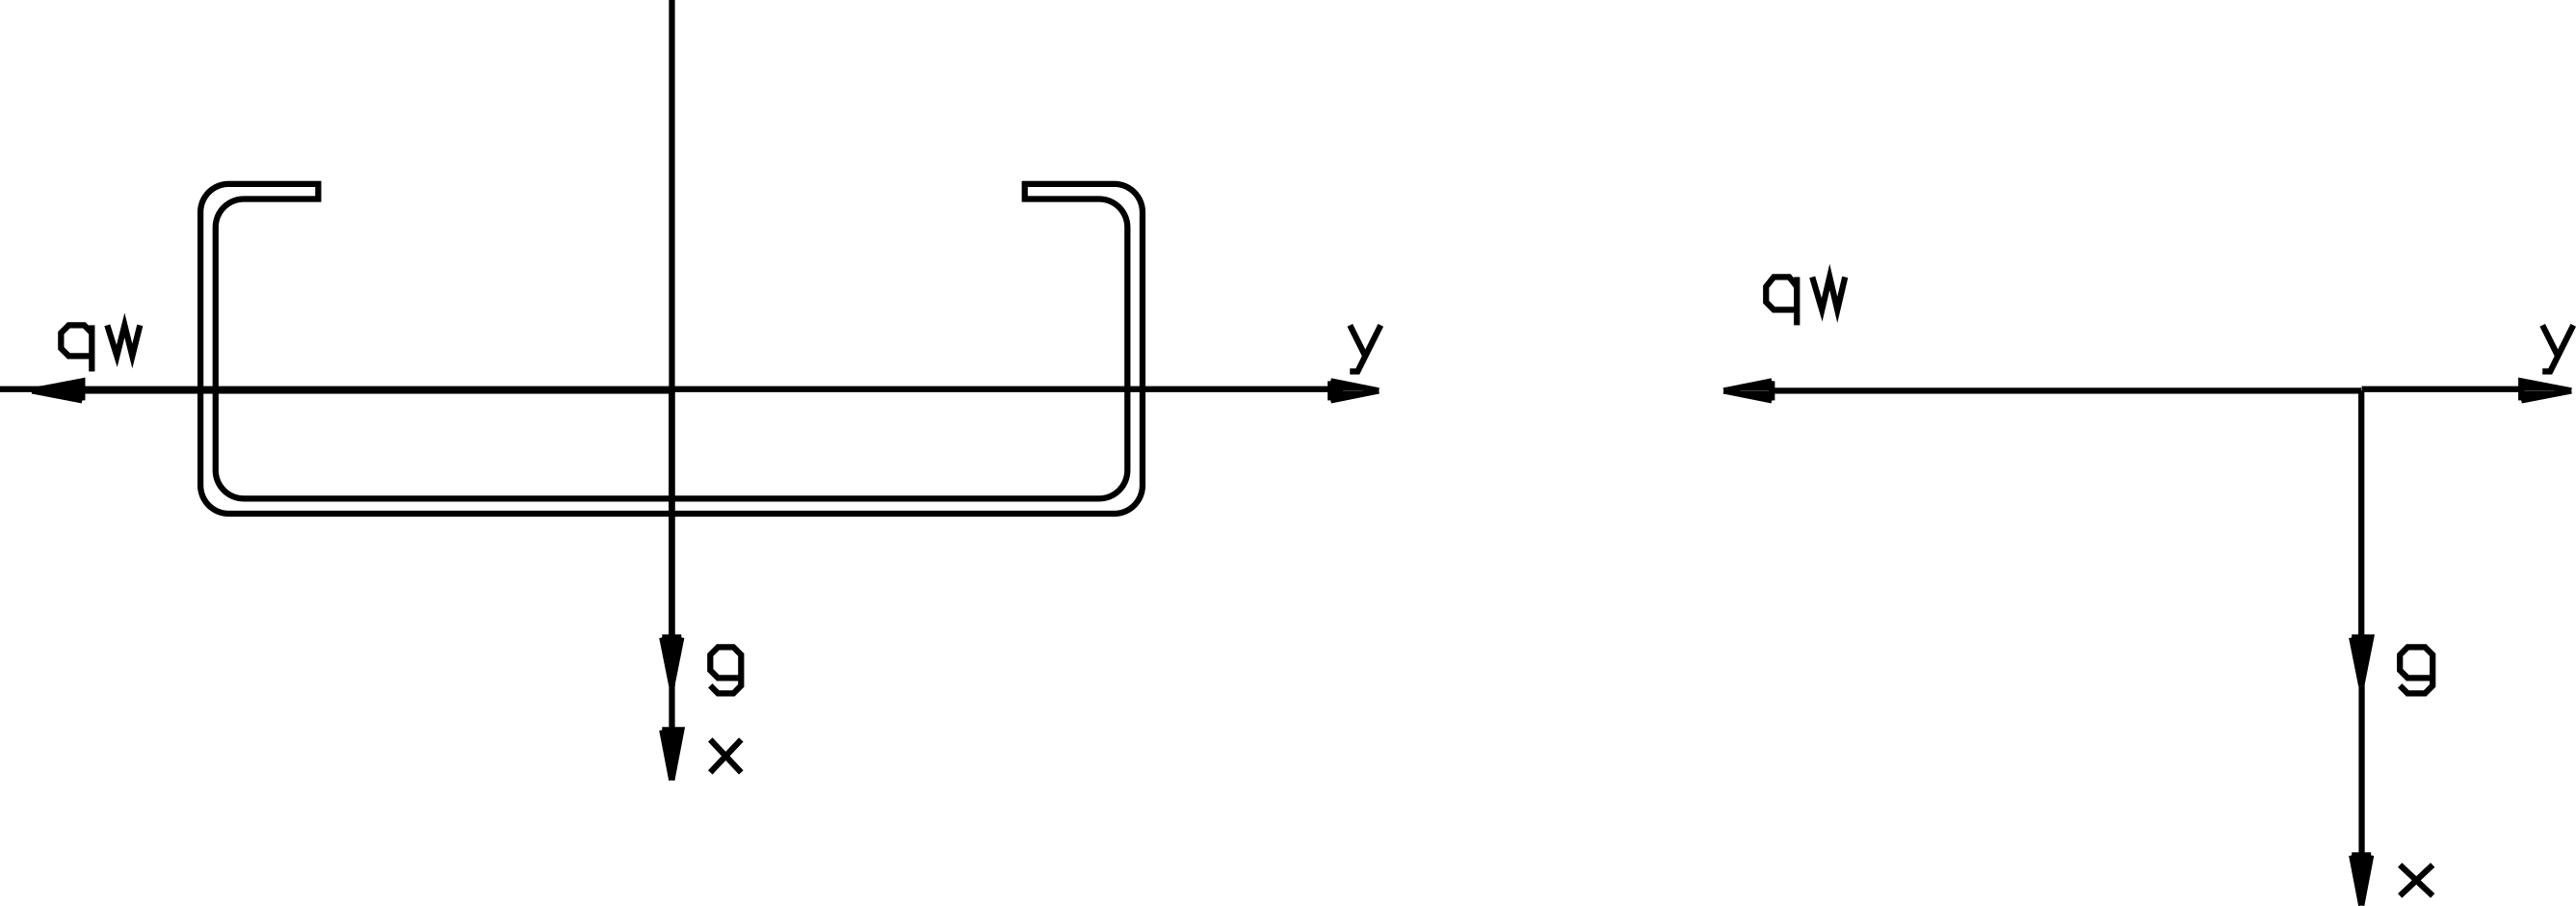
\includegraphics[scale = 1]{chapters/chapter_3/images/figura5.png}
\caption{Correa de pared - Estado: peso propio + viento}
\end{center}
\end{figure}

Descomponiendo la resultante en las direcciones $x$ e $y$ tenemos:
\begin{align*}
& \alpha = 90 \textsuperscript{o}\\
& q_x=g \cdot Sen \alpha \cdot s = 14 \frac{Kg}{m^2} \cdot 1.20m= \framebox{$16.8 \frac{Kg}{m}$}\\
& q_y=(q_w - g \cdot Cos \alpha) \cdot s = 214 \frac{Kg}{m^2} \cdot 1.20m= \framebox{$256.8 \frac{Kg}{m}$}
\end{align*}

Procedemos a calcular los momentos en el centro de la luz, producidos por cada una de estas cargas lineales, suponemos que las correas se encuentran simplemente apoyadas.

\begin{align*}
& M_x= \frac{q_y \cdot l^2}{8} = \frac{256.8 \frac{Kg}{m} \cdot (5m)^2}{8} = \framebox{$802.5 Kg.m$} \\
& M_y= \frac{q_x \cdot l^2}{8} = \frac{16.8 \frac{Kg}{m} \cdot (5m)^2}{8} = \framebox{$52.5 Kg.m$}
\end{align*}

\item Tension admisible.\\
Dado que se utiliza acero F-24, tenemos según el reglamento CIRSOC 301 una tensión de fluencia $\sigma_{fl}=2400 \frac{Kg}{cm^2}$ y tomando un coeficiente de seguridad $\gamma = 1.6$ , se obtiene una tensión admisible de:
$$\sigma_{adm}= \frac{\sigma_{fl}}{\gamma} = \frac{2400 \frac{Kg}{cm^2}}{1.6} = \framebox{$1500 \frac{Kg}{cm^2}$}$$

\item Selección de la correa.\\
Adoptamos un perfil \framebox{C 200-70-25-3.2} de chapa doblada, con las siguientes características:
\begin{align*}
& W_x= 70.448 cm^3 \\
& W_y= 16.057 cm^3 \\
& J_x= 704.478 cm^4 \\
& J_y= 78.006 cm^4
\end{align*}

\item Verificamos las tensiones para el estado de carga.\\
\underline{Estado de carga: peso propio + viento}
\begin{align*}
& \sigma_x=\frac{M_x}{W_x} = \frac{80250 Kg.cm}{70.448 cm^3} = 1139.13 \frac{Kg}{cm^2}\\
& \sigma_y=\frac{M_y}{W_y} = \frac{5250 Kg.cm}{16.057 cm^3} = 326.96 \frac{Kg}{cm^2}\\
& \sigma_t= \sigma_x + \sigma_y = 1139.13 \frac{Kg}{cm^2} + 326.96 \frac{Kg}{cm^2} = \framebox{$ 1466.09 \frac{Kg}{cm^2}$}\\
& \sigma_t < \sigma_{adm}\\
& 1466.09 \frac{Kg}{cm^2} < 1500 \frac{Kg}{cm^2} \Rightarrow \text{Verifica} \quad \surd
\end{align*}

\item Verificamos las deformaciones para el estado de carga.\\
La flecha admisible de cumplir $f < \frac{l}{300} \Rightarrow f < \frac{5m}{300} \Rightarrow f < 1.66cm$\\
Para el cálculo de la flecha utilizaremos la expresión $f= \frac{5}{384} \cdot \frac{q \cdot l^4}{E \cdot J}$\\

\underline{Estado de carga: peso propio + viento}
\begin{align*}
& f_x=\frac{5}{384} \cdot \frac{q_x \cdot l^4}{E \cdot J_y}\\
& f_x=\frac{5}{384} \cdot \frac{0.168 \frac{Kg}{cm} \cdot (500cm)^4}{2100000 \frac{Kg}{cm^2} \cdot 78.006 cm^4} = 0.835cm\\
& f_y=\frac{5}{384} \cdot \frac{q_y \cdot l^4}{E \cdot J_x}\\
& f_y=\frac{5}{384} \cdot \frac{2.568 \frac{Kg}{cm} \cdot (500cm)^4}{2100000 \frac{Kg}{cm^2} \cdot 704.478 cm^4} = 1.413cm\\
& f = \sqrt{f_x^2+f_y^2} = \sqrt{(0.835cm)^2+(1.413cm)^2} = \framebox{$1.64cm$}\\
& f < f_{adm}\\
& 1.64cm < 1.66cm \Rightarrow \text{Verifica} \quad \surd
\end{align*}
Por lo tanto verifica el requerimiento de deformación especificado en el reglamento.\\
\end{itemize}
\end{enumerate}